% Figura do Cap. II: períodos de otimização e de teste em linha do tempo.
% Substitui o Quadro "Períodos de otimização e de teste" desde 05/11/2026, a
% pedido do autor. Compilada pelo Makefile do tg/. Cópia de
% ia/relatorios/figuras-cap2/fig07-periodos.tex (o relatório usa a mesma).
% Procedência das datas:
%   otimização C1 a C4 e testes T1 a T3: tabela do
%     dados/resultados/refeito_2026-10-05/PROTOCOLO.md (datas do testador);
%   2017 a 2024: primeira e última linha de
%     dados/resultados/refeito_2026-10-05/testes/curva_R6_GS.csv;
%   sem as configurações fixas desde 05/11/2026 (pedido do autor: ficam só como
%     testes adicionais no Cap. III);
%   faixas de 2008 e 2020: anos-calendário dos recortes do Cap. III
%     (recorte_2008.txt e recorte_2020.txt).
\documentclass[10pt,border=2pt]{standalone}
\usepackage[T1]{fontenc}
\usepackage[utf8]{inputenc}
\usepackage{mathptmx}
\usepackage{tikz}
\usetikzlibrary{arrows.meta,patterns}
% posição horizontal de uma data: 0,5 cm por ano a partir de 01/01/2004
\newcommand{\X}[3]{\fpeval{0.5*((#1-2004) + (#2-1)/12 + (#3-1)/365)}}
\tikzset{
  otim/.style={draw, semithick, fill=gray!60, minimum height=5mm},
  teste/.style={draw, semithick, fill=gray!12, minimum height=5mm},
  txt/.style={font=\footnotesize, inner sep=1pt},
}
% \barra{linha}{estilo}{a1}{m1}{d1}{a2}{m2}{d2}{texto}
\newcommand{\barra}[9]{%
  \filldraw[#2] (\X{#3}{#4}{#5}, #1-0.25) rectangle (\X{#6}{#7}{#8}, #1+0.25);
  \node[txt] at ({(\X{#3}{#4}{#5}+\X{#6}{#7}{#8})/2}, #1) {#9};}
\begin{document}
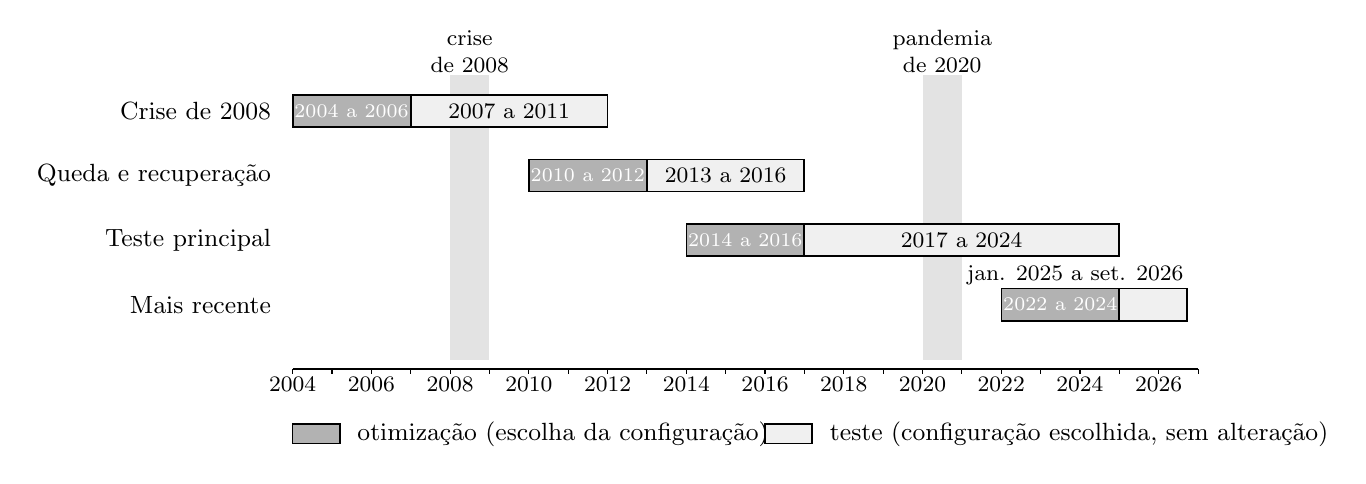
\begin{tikzpicture}[y=0.82cm]
  % faixas dos anos de crise analisados à parte no Cap. III
  \fill[gray!22] (\X{2008}{1}{1}, -3.85) rectangle (\X{2009}{1}{1}, 0.55);
  \fill[gray!22] (\X{2020}{1}{1}, -3.85) rectangle (\X{2021}{1}{1}, 0.55);
  \node[txt, above, align=center] at ({\X{2008}{7}{1}}, 0.55) {crise\\de 2008};
  \node[txt, above, align=center] at ({\X{2020}{7}{1}}, 0.55) {pandemia\\de 2020};

  % rótulos das linhas
  \foreach \y/\r in {0/{Crise de 2008}, -1/{Queda e recuperação}, -2/{Teste principal},
                     -3/{Mais recente}}
    \node[anchor=east, font=\small] at (-0.15, \y) {\r};

  % escolha refeita para cada teste, com os três anos anteriores
  \barra{0}{otim}{2004}{1}{2}{2006}{12}{29}{\scriptsize\color{white}2004 a 2006}
  \barra{0}{teste}{2007}{1}{2}{2011}{12}{30}{2007 a 2011}
  \barra{-1}{otim}{2010}{1}{4}{2012}{12}{28}{\scriptsize\color{white}2010 a 2012}
  \barra{-1}{teste}{2013}{1}{2}{2016}{12}{30}{2013 a 2016}
  \barra{-2}{otim}{2014}{1}{2}{2016}{12}{30}{\scriptsize\color{white}2014 a 2016}
  \barra{-2}{teste}{2017}{1}{2}{2024}{12}{27}{2017 a 2024}
  \barra{-3}{otim}{2022}{1}{3}{2024}{12}{30}{\scriptsize\color{white}2022 a 2024}
  \barra{-3}{teste}{2025}{1}{2}{2026}{9}{18}{}
  \node[txt, anchor=south east] at ({\X{2026}{9}{18}}, -2.75) {jan. 2025 a set. 2026};

  % eixo dos anos
  \draw[semithick] (0, -4) -- (\X{2027}{1}{1}, -4);
  \foreach \a in {2004,...,2027} \draw (\X{\a}{1}{1}, -4) -- ++(0, -0.08);
  \foreach \a in {2004,2006,...,2026}
    \node[txt, below] at (\X{\a}{1}{1}, -4.08) {\a};

  % legenda
  \begin{scope}[shift={(\X{2004}{1}{1}, -5.0)}]
    \filldraw[otim] (0, -0.15) rectangle (0.6, 0.15);
    \node[anchor=west, font=\small] at (0.7, 0) {otimização (escolha da configuração)};
    \filldraw[teste] (6.0, -0.15) rectangle (6.6, 0.15);
    \node[anchor=west, font=\small] at (6.7, 0) {teste (configuração escolhida, sem alteração)};
  \end{scope}
\end{tikzpicture}
\end{document}
